% D flip-flops (DFFs) and shift register
% Author: Martin Scharrer
\documentclass[a4paper,landscape]{article}

\usepackage{booktabs}
\usepackage{graphicx}
\usepackage{tikz}
\usepackage{url}
\usepackage{pgfplots}
\usepackage{hyperref}
\usepackage{pmboxdraw}
\usepackage{float}
\usepackage{listings}
\usepackage{circuitikz}
% Important: If latex complains about unicode characters,
% please use "\usepackage[utf8x]{inputenc}" in your preamble
% You can change the size of the picture by putting it into the construct:
% 1) \resizebox{10cm}{!}{"below picture"} to scale horizontally to 10 cm
% 2) \resizebox{!}{15cm}{"below picture"} to scale vertically to 15 cm
% 3) \resizebox{10cm}{15cm}{"below picture"} a combination of above two
% It is not recomended to use the scale option of the tikzpicture environment.
\centering
\resizebox{12cm}{!}{
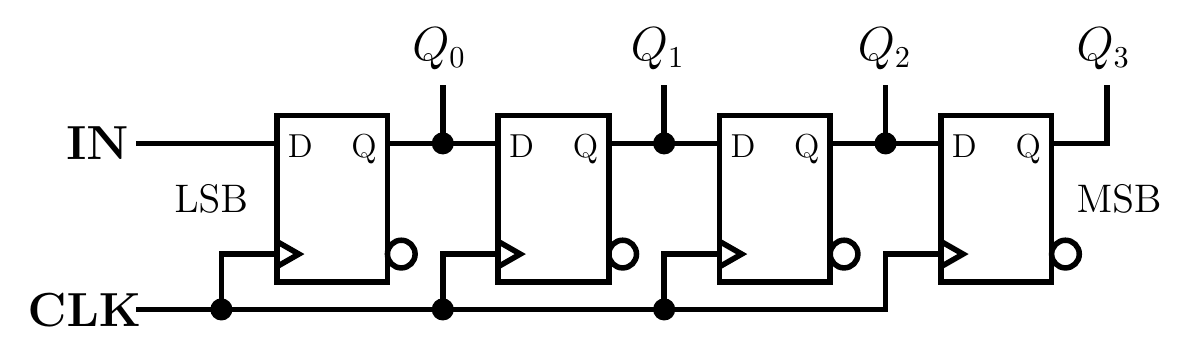
\begin{tikzpicture}[x=1pt,y=-1pt,line cap=rect]
  \def\logisimfontA#1{\fontfamily{cmr}{#1}} % Replaced by logisim, original font was "SansSerif"
  \definecolor{custcol_0_0_0}{RGB}{0, 0, 0}
  \definecolor{custcol_ff_ff_ff}{RGB}{255, 255, 255}
  \definecolor{custcol_80_80_80}{RGB}{128, 128, 128}
  \draw [line width=2.0pt, custcol_0_0_0 ]  (158.0,117.0) -- (238.0,117.0) -- (238.0,97.0) -- (248.0,97.0) ;
  \draw [line width=2.0pt, custcol_0_0_0 ]  (48.0,117.0) -- (78.0,117.0) -- (78.0,97.0) -- (88.0,97.0) ;
  \draw [line width=2.0pt, custcol_0_0_0 ]  (238.0,117.0) -- (318.0,117.0) -- (318.0,97.0) -- (328.0,97.0) ;
  \draw [line width=2.0pt, custcol_0_0_0 ]  (78.0,117.0) -- (158.0,117.0) -- (158.0,97.0) -- (168.0,97.0) ;
  \fill [line width=2.0pt, custcol_0_0_0]  (318.0,57.0) ellipse (4.0 and 4.0 );
  \fill [line width=2.0pt, custcol_0_0_0]  (238.0,117.0) ellipse (4.0 and 4.0 );
  \fill [line width=2.0pt, custcol_0_0_0]  (238.0,57.0) ellipse (4.0 and 4.0 );
  \fill [line width=2.0pt, custcol_0_0_0]  (158.0,117.0) ellipse (4.0 and 4.0 );
  \fill [line width=2.0pt, custcol_0_0_0]  (158.0,57.0) ellipse (4.0 and 4.0 );
  \fill [line width=2.0pt, custcol_0_0_0]  (78.0,117.0) ellipse (4.0 and 4.0 );
  \draw [line width=2.0pt, custcol_0_0_0 ]  (98.0,47.0) -- (137.0,47.0) ;
  \draw [line width=2.0pt, custcol_0_0_0 ]  (138.0,47.0) -- (138.0,106.0) ;
  \draw [line width=2.0pt, custcol_0_0_0 ]  (138.0,107.0) -- (99.0,107.0) ;
  \draw [line width=2.0pt, custcol_0_0_0 ]  (98.0,107.0) -- (98.0,48.0) ;

  \draw [line width=2.0pt, custcol_0_0_0 ]  (48.0,57.0) -- (88.0,57.0) -- (97.0,57.0) ;
  \logisimfontA{\fontsize{12pt}{12pt}\selectfont\node[inner sep=0, outer sep=0, custcol_0_0_0, anchor=base west] at  (102.0,62.0)  {D};}
  \draw [line width=2.0pt, custcol_0_0_0 ]  (99.0,93.0) -- (106.0,97.0) -- (99.0,101.0) ;
  \draw [line width=2.0pt, custcol_0_0_0 ]  (88.0,97.0) -- (97.0,97.0) ;
  \draw [line width=2.0pt, custcol_0_0_0 ]  (139.0,57.0) -- (148.0,57.0) -- (158.0,57.0) ;
  \logisimfontA{\fontsize{12pt}{12pt}\selectfont\node[inner sep=0, outer sep=0, custcol_0_0_0, anchor=base west] at  (125.0,62.0)  {Q};}
  \draw [line width=2.0pt, custcol_0_0_0]  (143.0,97.0) ellipse (5.0 and 5.0 );
  \draw [line width=2.0pt, custcol_0_0_0 ]  (178.0,47.0) -- (217.0,47.0) ;
  \draw [line width=2.0pt, custcol_0_0_0 ]  (218.0,47.0) -- (218.0,106.0) ;
  \draw [line width=2.0pt, custcol_0_0_0 ]  (218.0,107.0) -- (179.0,107.0) ;
  \draw [line width=2.0pt, custcol_0_0_0 ]  (178.0,107.0) -- (178.0,48.0) ;
  \draw [line width=2.0pt, custcol_0_0_0 ]  (158.0,37.0) -- (158.0,57.0) -- (168.0,57.0) -- (177.0,57.0) ;
  \logisimfontA{\fontsize{12pt}{12pt}\selectfont\node[inner sep=0, outer sep=0, custcol_0_0_0, anchor=base west] at  (182.0,62.0)  {D};}
  \draw [line width=2.0pt, custcol_0_0_0 ]  (179.0,93.0) -- (186.0,97.0) -- (179.0,101.0) ;
  \draw [line width=2.0pt, custcol_0_0_0 ]  (168.0,97.0) -- (177.0,97.0) ;
  \draw [line width=2.0pt, custcol_0_0_0 ]  (219.0,57.0) -- (228.0,57.0) -- (238.0,57.0) -- (238.0,37.0) ;
  \logisimfontA{\fontsize{12pt}{12pt}\selectfont\node[inner sep=0, outer sep=0, custcol_0_0_0, anchor=base west] at  (205.0,62.0)  {Q};}
  \draw [line width=2.0pt, custcol_0_0_0]  (223.0,97.0) ellipse (5.0 and 5.0 );
  \draw [line width=2.0pt, custcol_0_0_0 ]  (258.0,47.0) -- (297.0,47.0) ;
  \draw [line width=2.0pt, custcol_0_0_0 ]  (298.0,47.0) -- (298.0,106.0) ;
  \draw [line width=2.0pt, custcol_0_0_0 ]  (298.0,107.0) -- (259.0,107.0) ;
  \draw [line width=2.0pt, custcol_0_0_0 ]  (258.0,107.0) -- (258.0,48.0) ;
  \draw [line width=2.0pt, custcol_0_0_0 ]  (238.0,57.0) -- (248.0,57.0) -- (257.0,57.0) ;
  \logisimfontA{\fontsize{12pt}{12pt}\selectfont\node[inner sep=0, outer sep=0, custcol_0_0_0, anchor=base west] at  (262.0,62.0)  {D};}
  \draw [line width=2.0pt, custcol_0_0_0 ]  (259.0,93.0) -- (266.0,97.0) -- (259.0,101.0) ;
  \draw [line width=2.0pt, custcol_0_0_0 ]  (248.0,97.0) -- (257.0,97.0) ;
  \draw [line width=2.0pt, custcol_0_0_0 ]  (299.0,57.0) -- (308.0,57.0) -- (318.0,57.0) ;
  \logisimfontA{\fontsize{12pt}{12pt}\selectfont\node[inner sep=0, outer sep=0, custcol_0_0_0, anchor=base west] at  (285.0,62.0)  {Q};}
  \draw [line width=2.0pt, custcol_0_0_0]  (303.0,97.0) ellipse (5.0 and 5.0 );
  \draw [line width=2.0pt, custcol_0_0_0 ]  (338.0,47.0) -- (377.0,47.0) ;
  \draw [line width=2.0pt, custcol_0_0_0 ]  (378.0,47.0) -- (378.0,106.0) ;
  \draw [line width=2.0pt, custcol_0_0_0 ]  (378.0,107.0) -- (339.0,107.0) ;
  \draw [line width=2.0pt, custcol_0_0_0 ]  (338.0,107.0) -- (338.0,48.0) ;
  \draw [line width=2.0pt, custcol_0_0_0 ]  (318.0,37.0) -- (318.0,57.0) -- (328.0,57.0) -- (337.0,57.0) ;
  \logisimfontA{\fontsize{12pt}{12pt}\selectfont\node[inner sep=0, outer sep=0, custcol_0_0_0, anchor=base west] at  (342.0,62.0)  {D};}
  \draw [line width=2.0pt, custcol_0_0_0 ]  (339.0,93.0) -- (346.0,97.0) -- (339.0,101.0) ;
  \draw [line width=2.0pt, custcol_0_0_0 ]  (328.0,97.0) -- (337.0,97.0) ;
  \draw [line width=2.0pt, custcol_0_0_0 ]  (379.0,57.0) -- (388.0,57.0) -- (398.0,57.0) -- (398.0,37.0) ;
  \logisimfontA{\fontsize{12pt}{12pt}\selectfont\node[inner sep=0, outer sep=0, custcol_0_0_0, anchor=base west] at  (365.0,62.0)  {Q};}
  \draw [line width=2.0pt, custcol_0_0_0]  (383.0,97.0) ellipse (5.0 and 5.0 );
  \logisimfontA{\fontsize{16pt}{16pt}\fontseries{bx}\selectfont\node[inner sep=0, outer sep=0, custcol_0_0_0, anchor=base west] at  (8.0,123.0)  {CLK};}
  \logisimfontA{\fontsize{14pt}{14pt}\selectfont\node[inner sep=0, outer sep=0, custcol_0_0_0, anchor=base west] at  (61.0,82.0)  {LSB};}
  \logisimfontA{\fontsize{14pt}{14pt}\selectfont\node[inner sep=0, outer sep=0, custcol_0_0_0, anchor=base west] at  (387.0,82.0)  {MSB};}
  \logisimfontA{\fontsize{16pt}{16pt}\fontseries{bx}\selectfont\node[inner sep=0, outer sep=0, custcol_0_0_0, anchor=base west] at  (22.0,63.0)  {IN};}
  \logisimfontA{\fontsize{16pt}{16pt}\fontseries{bx}\selectfont\node[inner sep=0, outer sep=0, custcol_0_0_0, anchor=base west] at  (147.0,27.0)  {$Q_0$};}
  \logisimfontA{\fontsize{16pt}{16pt}\fontseries{bx}\selectfont\node[inner sep=0, outer sep=0, custcol_0_0_0, anchor=base west] at  (308.0,27.0)  {$Q_2$};}
  \logisimfontA{\fontsize{16pt}{16pt}\fontseries{bx}\selectfont\node[inner sep=0, outer sep=0, custcol_0_0_0, anchor=base west] at  (226.0,27.0)  {$Q_1$};}
  \logisimfontA{\fontsize{16pt}{16pt}\fontseries{bx}\selectfont\node[inner sep=0, outer sep=0, custcol_0_0_0, anchor=base west] at  (387.0,27.0)  {$Q_3$};}
  \end{tikzpicture}
}
  
    
\end{document}